% Each section is a new appendix
\section{Appendix A}\label{sec:vision_appendix_A}
% You can use how many "subsections" and "subsubsections" you like.

\begin{figure}[h]
	
\includegraphics[scale=0.5]{./figure/normal.jpg}
	\caption{Sample Input}
	\label{fig:normal output}
\end{figure}

\begin{figure}[h]
	
\includegraphics[scale=0.5]{./figure/negative.jpg}
	\caption{Invert Input}
	\label{fig:Invert output}
\end{figure}

\begin{figure}[h]
	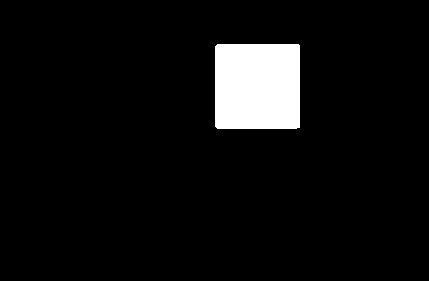
\includegraphics[scale=0.45]{./figure/mask.jpg}
	\caption{Sample Output for Red Threshold Masking}
	\label{fig:masking output}
\end{figure}

\begin{figure}[h]
	
\includegraphics[scale=0.5]{./figure/contours.jpg}
	\caption{Sample Output for Contour Tracing}
	\label{fig:contour output}
\end{figure}

\begin{figure}[h]
	
\includegraphics[scale=0.5]{./figure/canny.jpg}
	\caption{Sample Output for Canny Edge Detection}
	\label{fig:canny output}
\end{figure}
\pagebreak

\begin{figure}[h]
	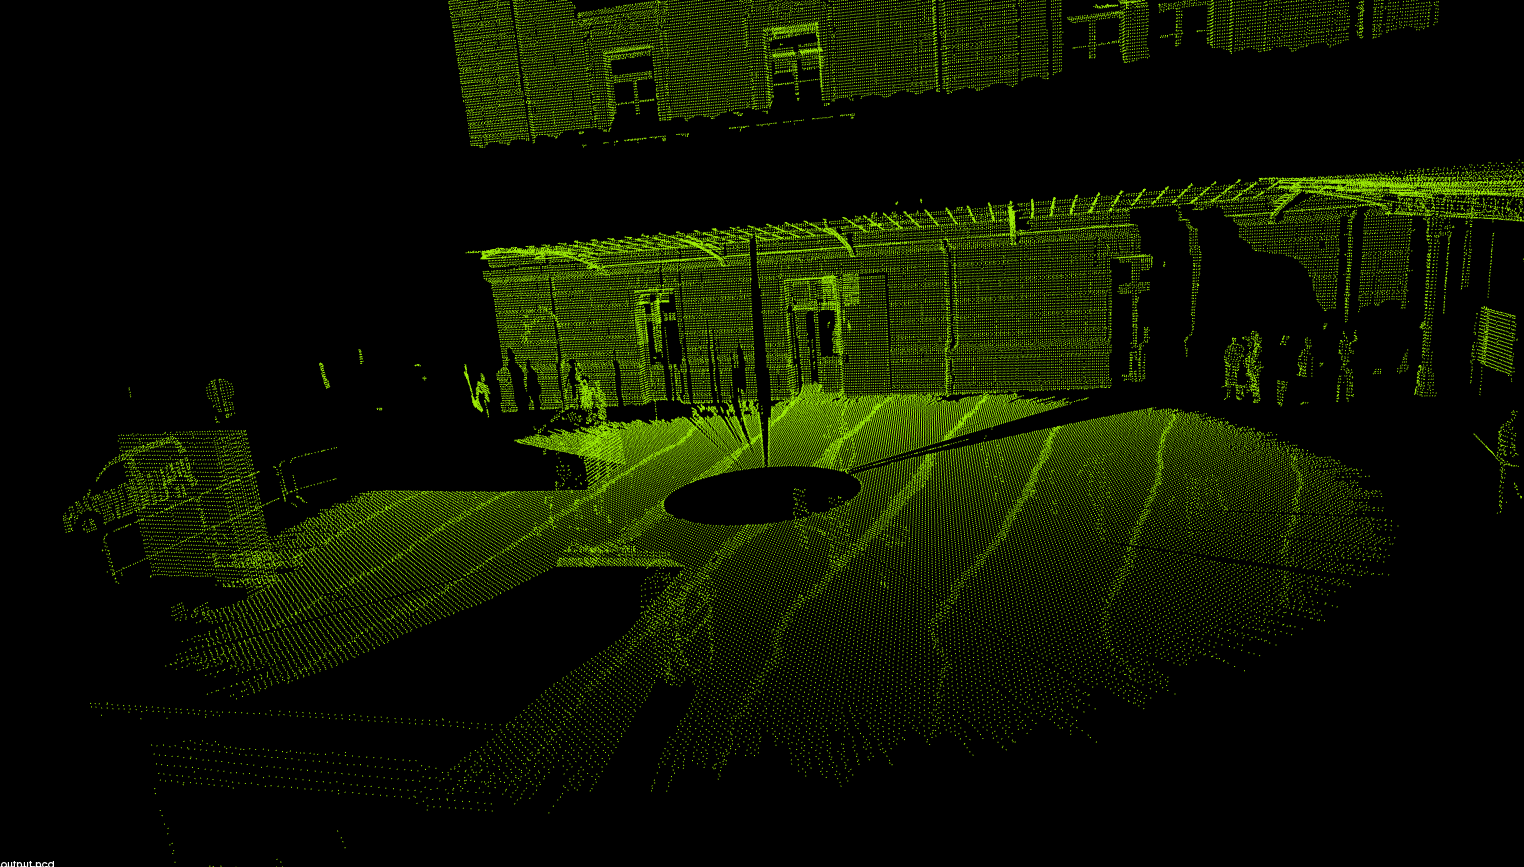
\includegraphics[width=0.5\textwidth]{./figure/statueBefore.png}
	\caption{Sample Input for Conditional Euclidean Segmentation}
	\label{fig:euclidean input}
\end{figure}

\begin{figure}[h]
	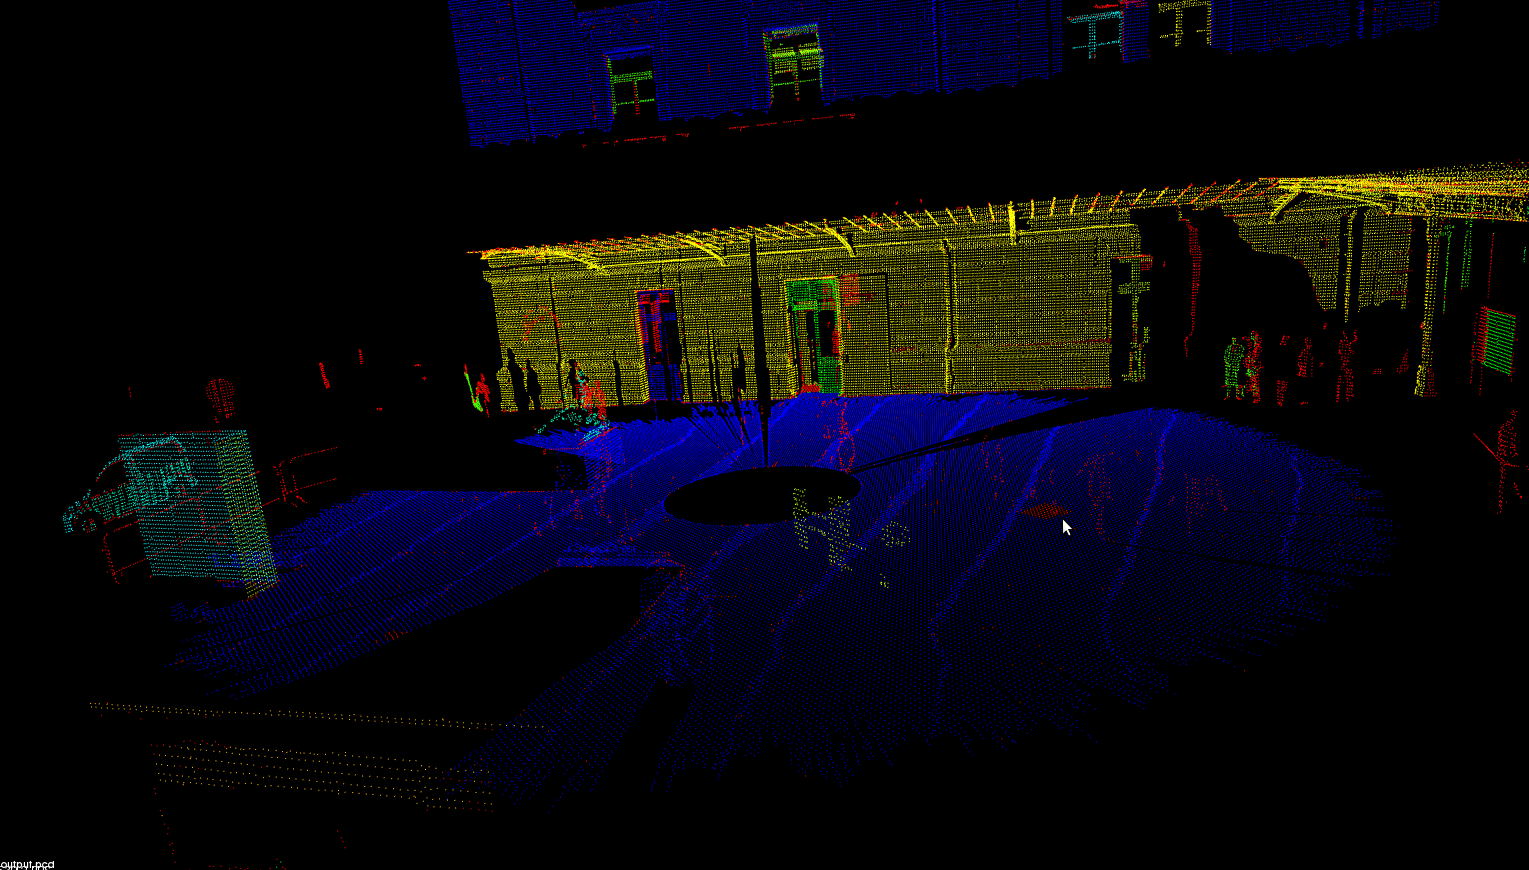
\includegraphics[width=0.5\textwidth]{./figure/statueAfter.png}
	\caption{Sample Output for Conditional Euclidean Segmentation}
	\label{fig:euclidean output}
\end{figure}

\begin{figure}[h]
	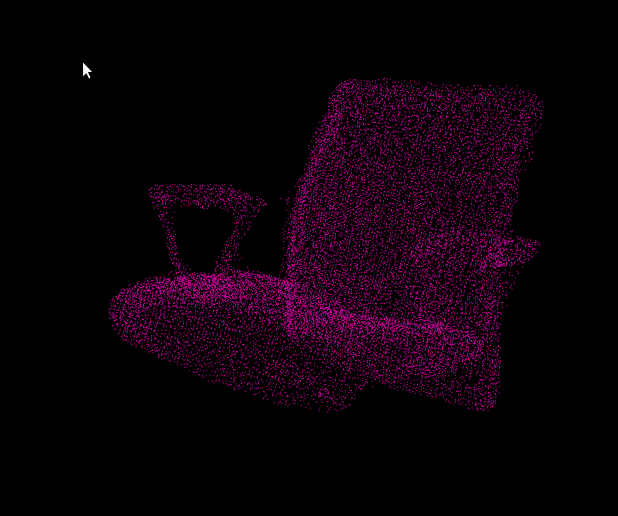
\includegraphics[width=0.5\textwidth]{./figure/pointChair.png}
	\caption{Sample Input PCL}
	\label{fig:Chair Point Cloud}
\end{figure}


\begin{figure}[h]
	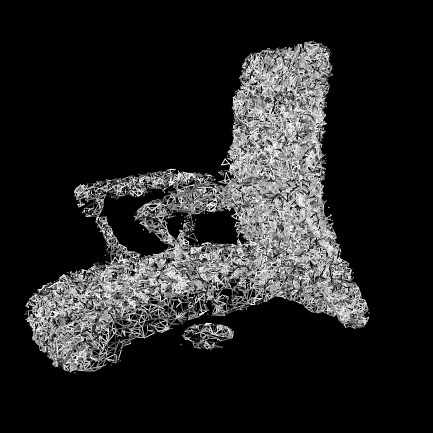
\includegraphics[width=0.5\textwidth]{./figure/meshChair.png}
	\caption{Sample Output for Greedy Triangulation Algorithm}
	\label{fig:greedy output}
\end{figure}

\begin{figure}[h]
	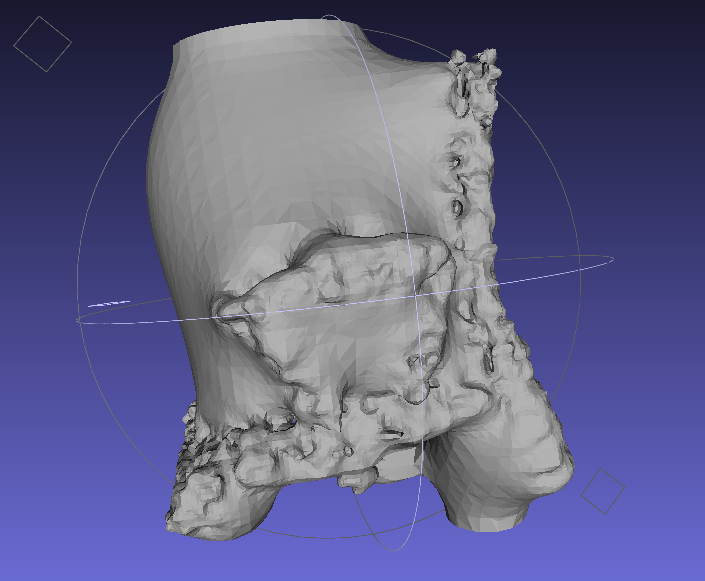
\includegraphics[width=0.5\textwidth]{./figure/poissonChair.png}
	\caption{Sample Output for Poisson Algorithm}
	\label{fig:poisson output}
\end{figure}